\newpage
% ============================================================
\section{Actividad 6: Fractalidad en tráfico transaccional Cloud y memoria institucional}
% ============================================================

% ------------------------------------------------------------
\subsection{Contexto: un arco transversal}
% ------------------------------------------------------------

El arco analítico desarrollado en las actividades previas sigue una progresión
metodológica deliberada. Las Actividades~1 y~2 validaron las propiedades
estadísticas de los estimadores Varianza--Tiempo y Log--Escala sobre secuencias
sintéticas de referencia: secuencias i.i.d.\ con $H=0{,}5$ como límite de
independencia, y procesos LRD monofractales (\texttt{wfbm}) y multifractales
(\texttt{betamwm}) como banco de prueba controlado. Las Actividades~3,~4 y~5
trasladaron estas herramientas al dominio fisiológico, caracterizando la
estructura fractal de la variabilidad cardíaca y construyendo un clasificador
mono/multifractal con asociaciones clínicas significativas.

La pregunta que orienta esta actividad es de naturaleza transversal: ¿la
fractalidad es un fenómeno exclusivo de sistemas biológicos, o emerge también en
infraestructuras tecnológicas? A diferencia de la fisiología cardíaca, donde la
regulación autónoma produce memoria persistente con $H\approx0{,}96$ y
heterogeneidad multiescala, el tráfico transaccional Cloud opera bajo dinámicas
de usuarios concurrentes, cachés en cascada y ráfagas de solicitudes
correlacionadas. Este hallazgo trasciende el dominio tecnológico: si la
fractalidad aparece tanto en un corazón sano como en un servidor web bajo carga,
debe existir un conjunto de propiedades estructurales comunes que la generen.

Para enriquecer esta perspectiva transversal, se incorpora un tercer dominio de
aplicación: las tasas de interés soberanas de Estados Unidos (serie DGS10 de
FRED). Este sistema financiero representa una instancia de ``memoria
institucional'', donde las decisiones de política monetaria, la persistencia de
shocks macroeconómicos y la suavización deliberada de las autoridades monetarias
generan dependencia de rango largo de intensidad intermedia entre la tecnología
y la biología. La inclusión del DGS10 transforma la taxonomía de un ``punto
tecnológico aislado'' en un \textbf{gradiente continuo} de memoria persistente.

% ------------------------------------------------------------
\subsection{Dataset y metodología: tráfico NASA HTTP}
% ------------------------------------------------------------

Se analiza el dataset NASA HTTP, un registro de solicitudes HTTP al servidor web
de la NASA durante los meses de julio y agosto de 1995. La serie objeto de
estudio son los tiempos entre llegadas consecutivas (\textit{inter-arrival
times}), que capturan la dinámica de acceso de miles de usuarios concurrentes.

La serie contiene $975\,721$ muestras con media $\mu = 2{,}7450\,\text{s}$,
mediana $1{,}0000\,\text{s}$ y desviación estándar
$\sigma = 137{,}6685\,\text{s}$. La enorme dispersión (coeficiente de
variación $>50$) es indicio de heterogeneidad estructural: la mayoría de los
intervalos son breves, pero episodios de congestión producen colas de espera de
varios minutos.

\begin{figure}[H]
    \centering
    \begin{minipage}[t]{0.48\textwidth}
        \centering
        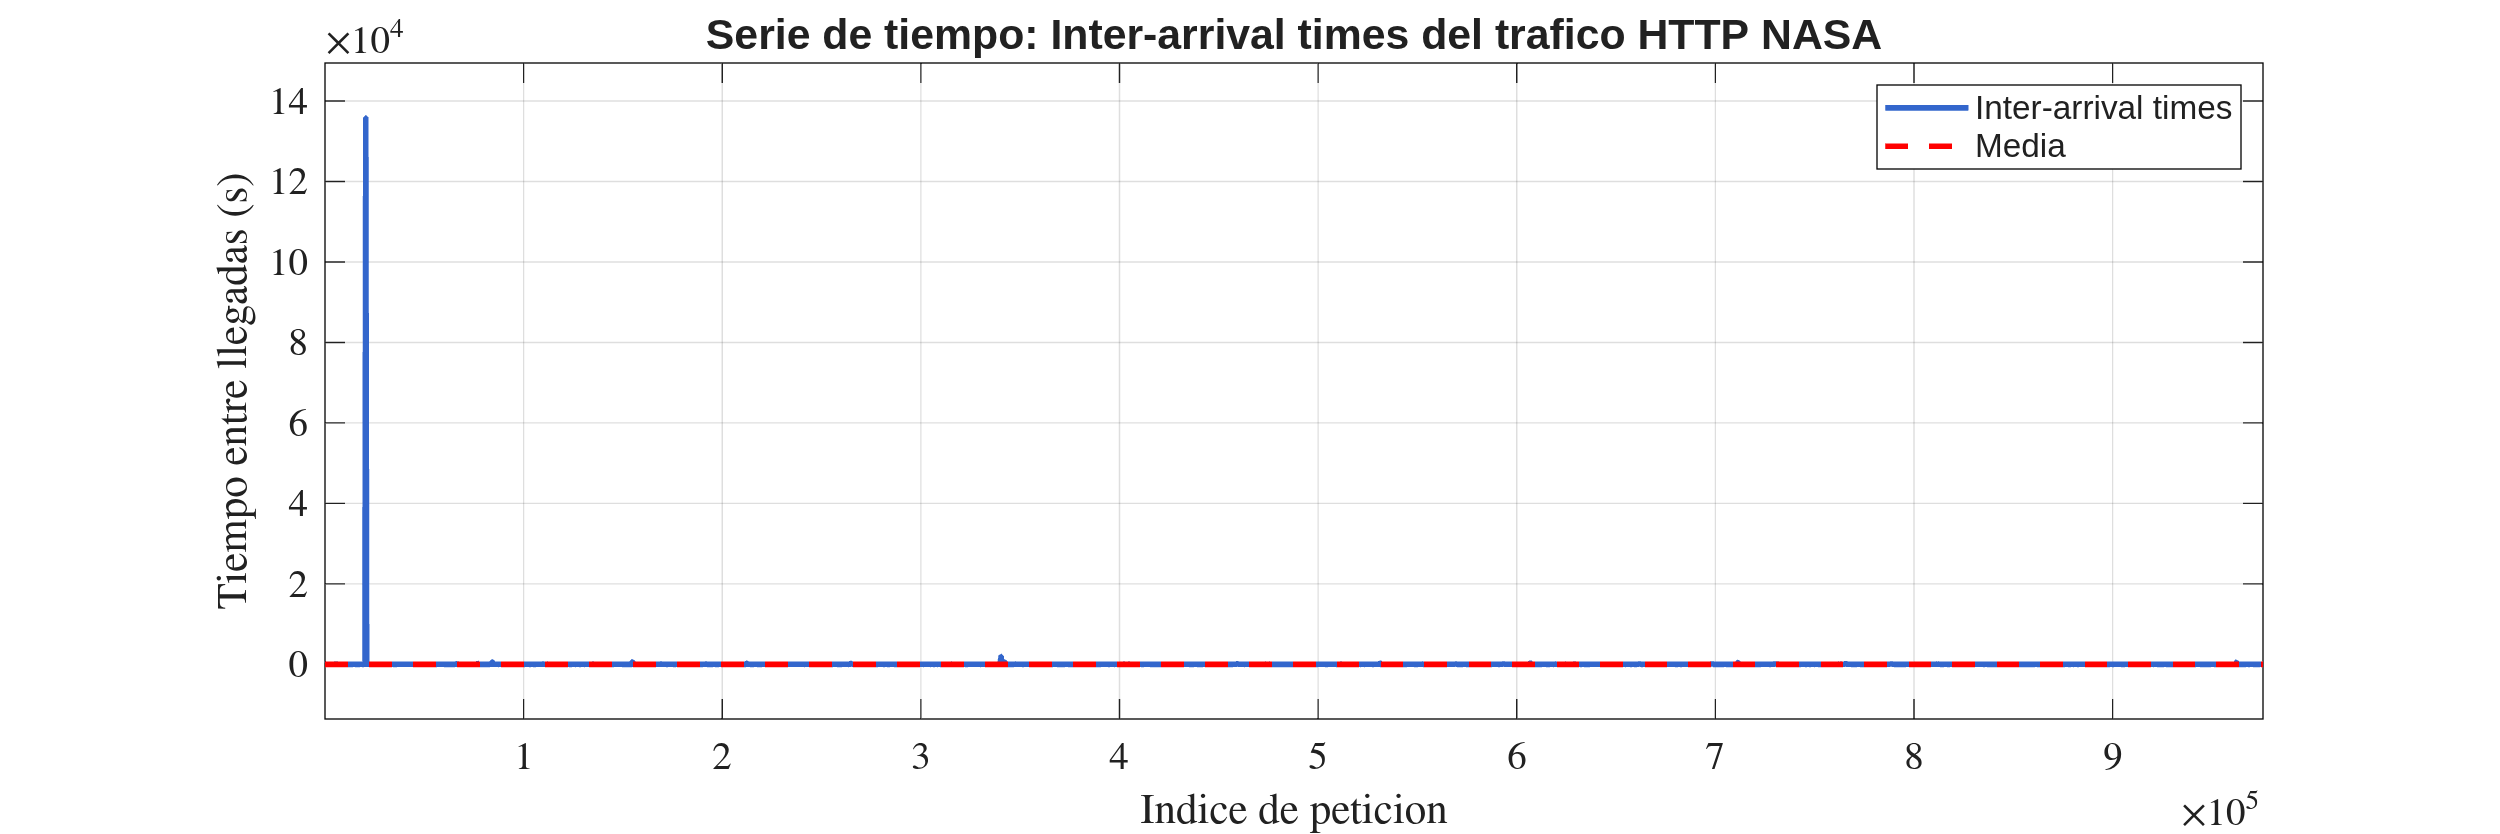
\includegraphics[width=\textwidth]{actividades/actividad6/imgs/serie_tiempo.png}
        \caption{Serie de tiempos entre llegadas del dataset NASA HTTP.
                 Se observan ráfagas intensas seguidas de periodos de
                 actividad reducida.}
        \label{fig:a6-serie}
    \end{minipage}
    \hfill
    \begin{minipage}[t]{0.48\textwidth}
        \centering
        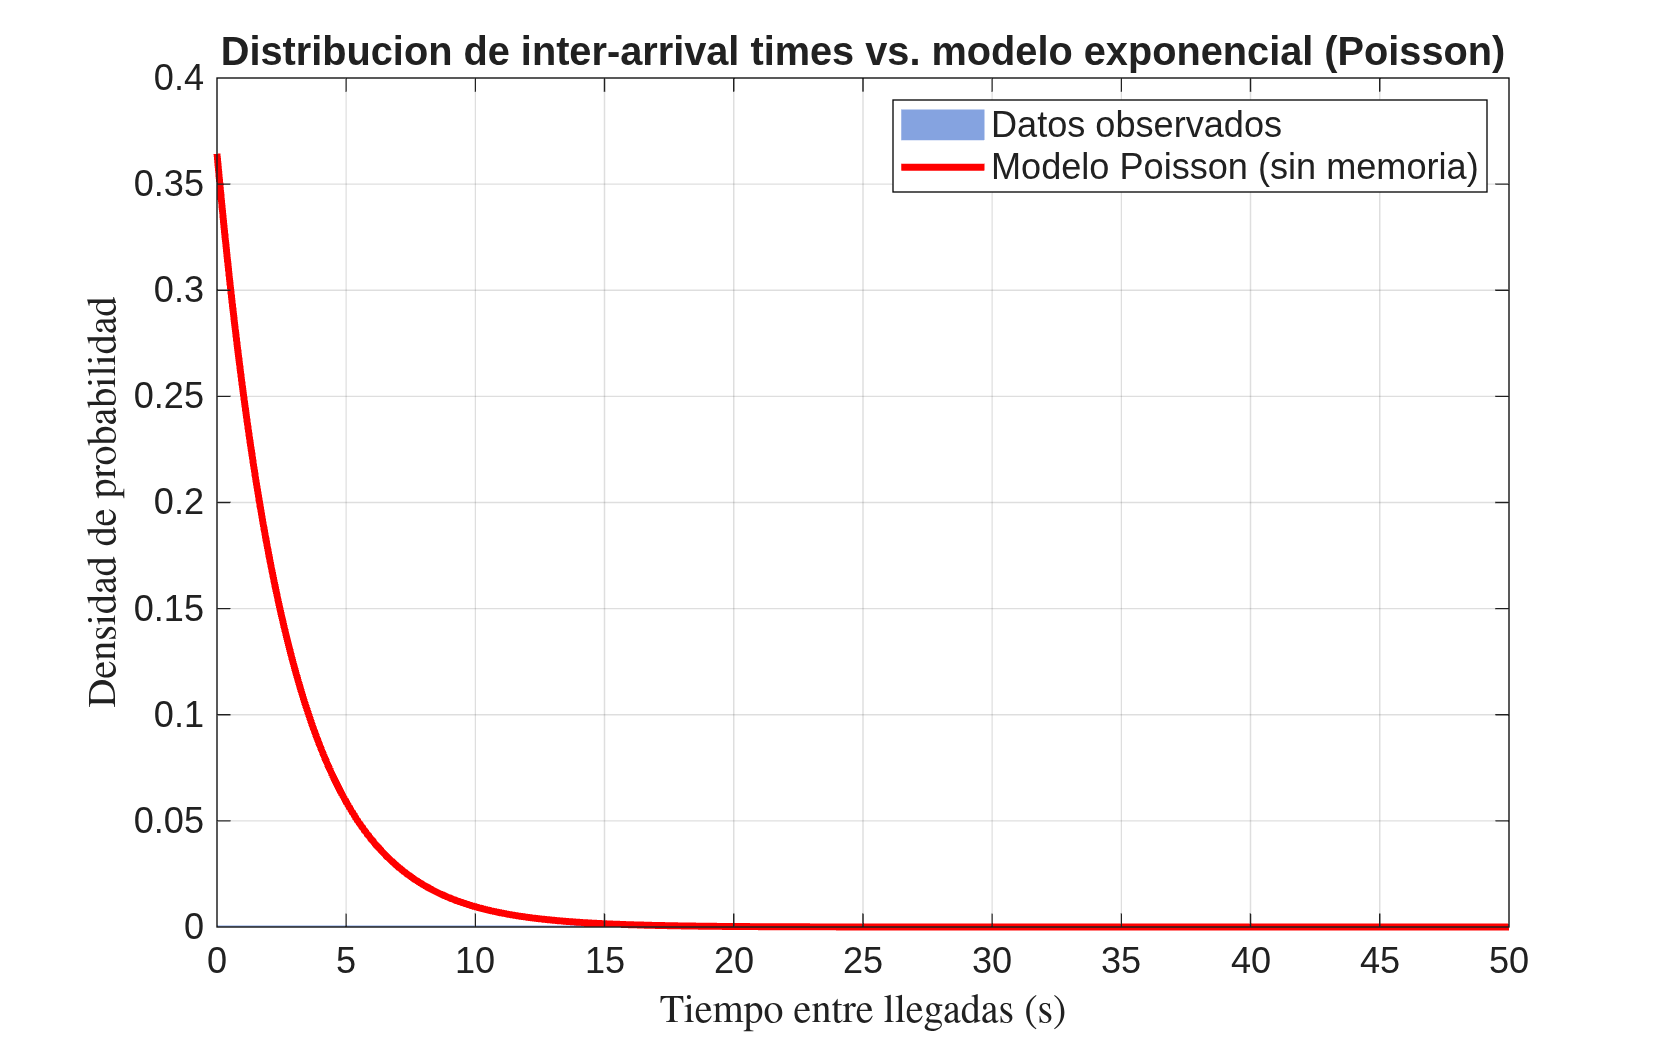
\includegraphics[width=\textwidth]{actividades/actividad6/imgs/histograma.png}
        \caption{Histograma de los inter-arrival times. La cola pesada
                 refleja la presencia de eventos de larga duración.}
        \label{fig:a6-hist}
    \end{minipage}
\end{figure}

Los estimadores VT y LD, así como el clasificador de la Actividad~4, se aplican
sin modificación metodológica, garantizando comparabilidad con los dominios
previos. Esta continuidad metodológica es esencial: permite situar el tráfico
NASA en el mismo espacio de parámetros que las secuencias sintéticas y las
señales cardíacas.

% ------------------------------------------------------------
\subsection{Dataset complementario: deuda soberana}
% ------------------------------------------------------------

Como complemento al benchmark tecnológico, se incorpora la serie \textbf{DGS10}
del repositorio FRED (Federal Reserve Economic Data): el rendimiento diario de
los bonos del Tesoro de Estados Unidos a 10 años de madurez constante. Esta
serie constituye el activo de referencia (\textit{risk-free rate}) del sistema
financiero global y captura la trayectoria de las expectativas de inflación,
crecimiento y política monetaria a largo plazo.

El dataset fue descargado mediante el script \texttt{src/descarga\_fred.py} y
preprocesado para eliminar valores faltantes mediante interpolación lineal. La
serie en niveles abarca $n = 16\,801$ observaciones diarias desde el
2 de enero de 1962 hasta el 26 de mayo de 2026, cubriendo más de seis décadas
que incluyen múltiples ciclos económicos, crisis financieras y cambios de
régimen monetario.

\begin{table}[H]
\centering
\caption{Estadísticas descriptivas del dataset FRED DGS10.}
\label{tab:dgs10-stats}
\begin{tabular}{lcc}
\toprule
\textbf{Estadística} & \textbf{Niveles (\%)} & \textbf{Diferencias diarias (pp)} \\
\midrule
Muestras & $16\,801$ & $16\,801$ \\
Media & $5{,}8139$ & $-0{,}0004$ \\
Mediana & $5{,}4300$ & $0{,}0000$ \\
Desv.~estándar & $2{,}9353$ & $0{,}0689$ \\
Mínimo & $0{,}5200$ & $-0{,}3300$ \\
Máximo & $15{,}8400$ & $0{,}4700$ \\
$\text{ACF}(1)$ & $\mathbf{0{,}9998}$ & $0{,}0284$ \\
\bottomrule
\end{tabular}
\end{table}

La autocorrelación de primer orden en niveles, $\text{ACF}(1)=0{,}9998$, es un
indicador contundente de memoria persistente. En contraste, las diferencias
diarias exhiben $\text{ACF}(1)\approx0{,}03$, lo que sugiere que la serie en
niveles es altamente integrada y que su estructura fractal reside en la
dinámica de largo plazo, no en los incrementos de corto plazo. Esta propiedad
es consistente con la literatura empírica sobre tasas de interés soberanas,
donde la suavización de política monetaria y la persistencia de shocks
macroeconómicos generan dependencia de rango largo con $H$ esperado en el
intervalo $0{,}65$--$0{,}85$
\cite{backus1993long,mcarthur1995hurst,bariviera2018efficiency}.

\begin{figure}[H]
    \centering
    \begin{minipage}[t]{0.48\textwidth}
        \centering
        \fbox{\parbox[c][0.25\textheight][c]{0.9\textwidth}{\centering
            \texttt{[Placeholder: serie\_tiempo\_dgs10.png]}\\[1ex]
            Serie diaria DGS10 (1962--2026).
        }}
        \caption{Evolución histórica del rendimiento del Tesoro a 10 años.
                 Se distinguen los ciclos de alta inflación (1970--80),
                 la Gran Moderación (1990--2000) y el régimen de tasas
                 bajas post-2008.}
        \label{fig:a6-dgs10-serie}
    \end{minipage}
    \hfill
    \begin{minipage}[t]{0.48\textwidth}
        \centering
        \fbox{\parbox[c][0.25\textheight][c]{0.9\textwidth}{\centering
            \texttt{[Placeholder: histograma\_dgs10.png]}\\[1ex]
            Histograma de niveles DGS10.
        }}
        \caption{Distribución empírica de los niveles DGS10. La forma
                 bimodal leve refleja los dos regímenes de tasas altas
                 y bajas predominantes en la muestra.}
        \label{fig:a6-dgs10-hist}
    \end{minipage}
\end{figure}

% ------------------------------------------------------------
\subsection{Estimación del parámetro de Hurst: tráfico NASA}
% ------------------------------------------------------------

El método Varianza--Tiempo arroja $\hat{H}_{\text{VT}}^{\text{(NASA)}} = 0{,}5435$ con
$R^2_{\text{VT}} = 0{,}9911$ e intervalo de confianza del $95\%$
$[0{,}5408;\,0{,}5462]$. El ajuste lineal del diagrama log-log es excelente,
confirmando que el escalamiento de varianza sigue una ley de potencias
consistente con dependencia de rango largo ($H > 0{,}5$).

El método Log--Escala obtiene $\hat{H}_{\text{LD}}^{\text{(NASA)}} = 0{,}5064$ con parámetro de
escala $\alpha = 0{,}0127$. La estimación es más conservadora que VT, en línea
con los hallazgos de las Actividades~1 y~3, donde LD exhibió mayor varianza en
muestras de gran tamaño con alta LRD.

\begin{figure}[H]
    \centering
    \begin{minipage}[t]{0.48\textwidth}
        \centering
        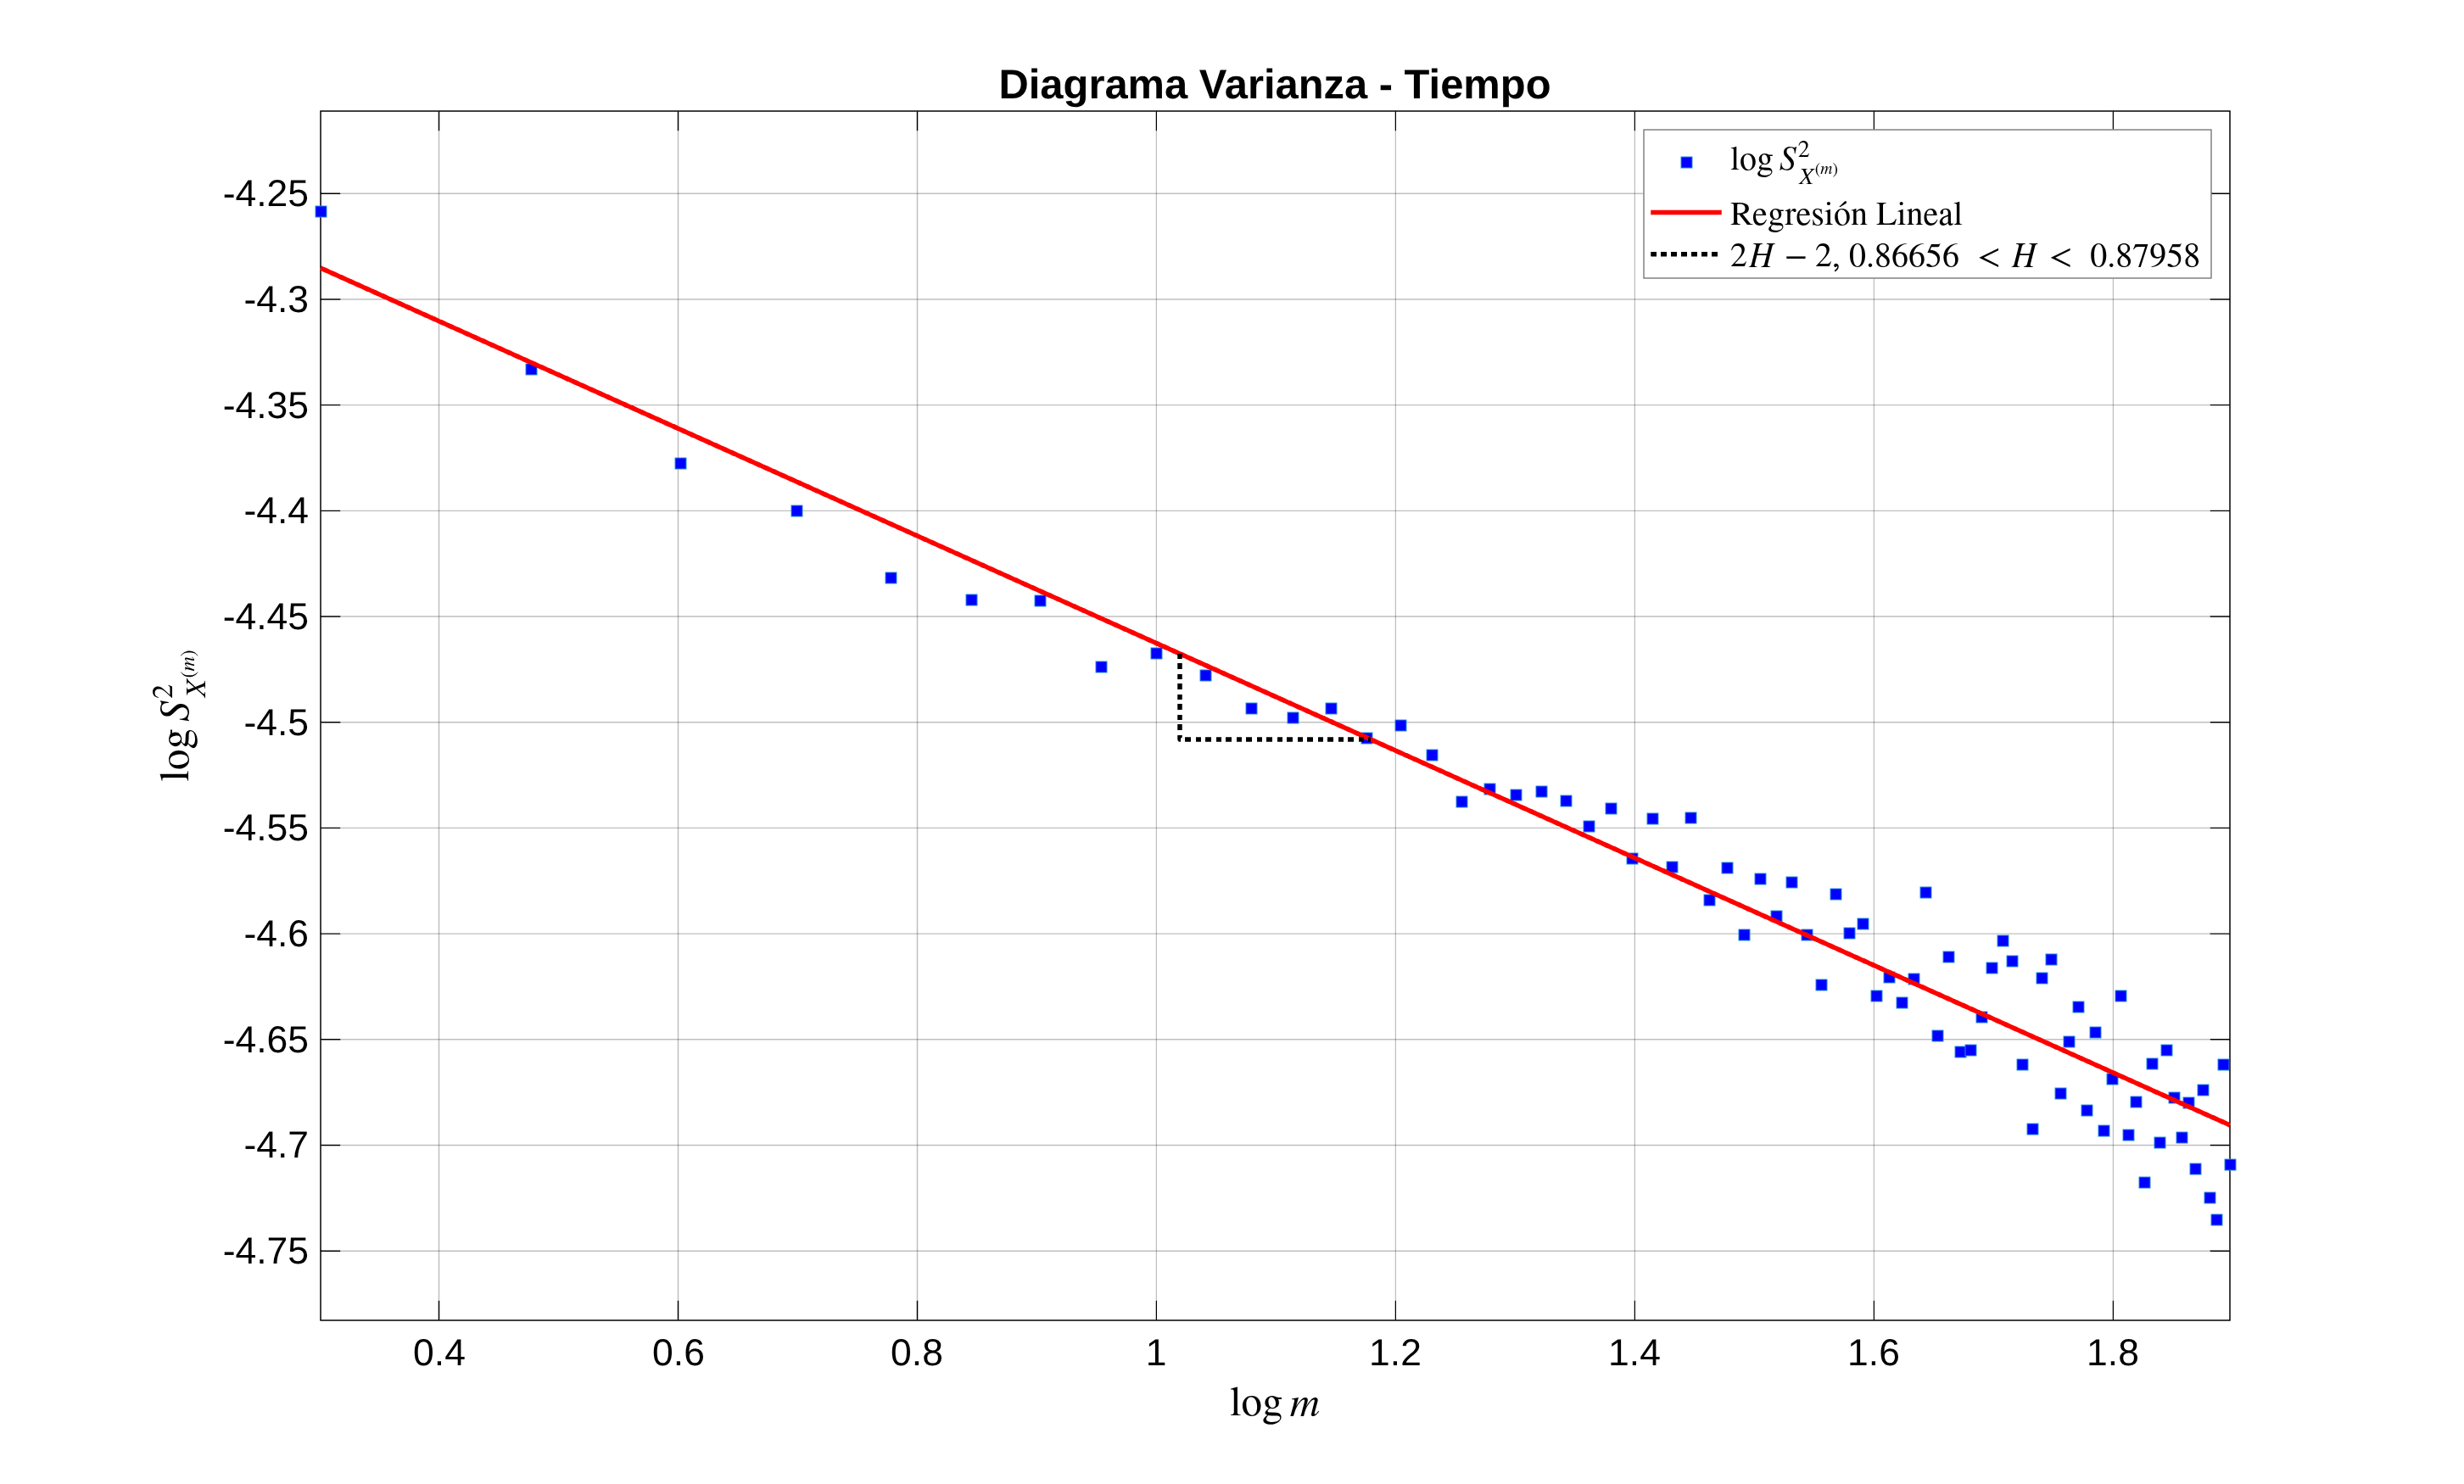
\includegraphics[width=\textwidth]{actividades/actividad6/imgs/diagrama_vt.png}
        \caption{Diagrama Varianza--Tiempo (NASA). La pendiente del ajuste lineal
                 determina $\hat{H} = 0{,}5435$, confirmando LRD.}
        \label{fig:a6-vt}
    \end{minipage}
    \hfill
    \begin{minipage}[t]{0.48\textwidth}
        \centering
        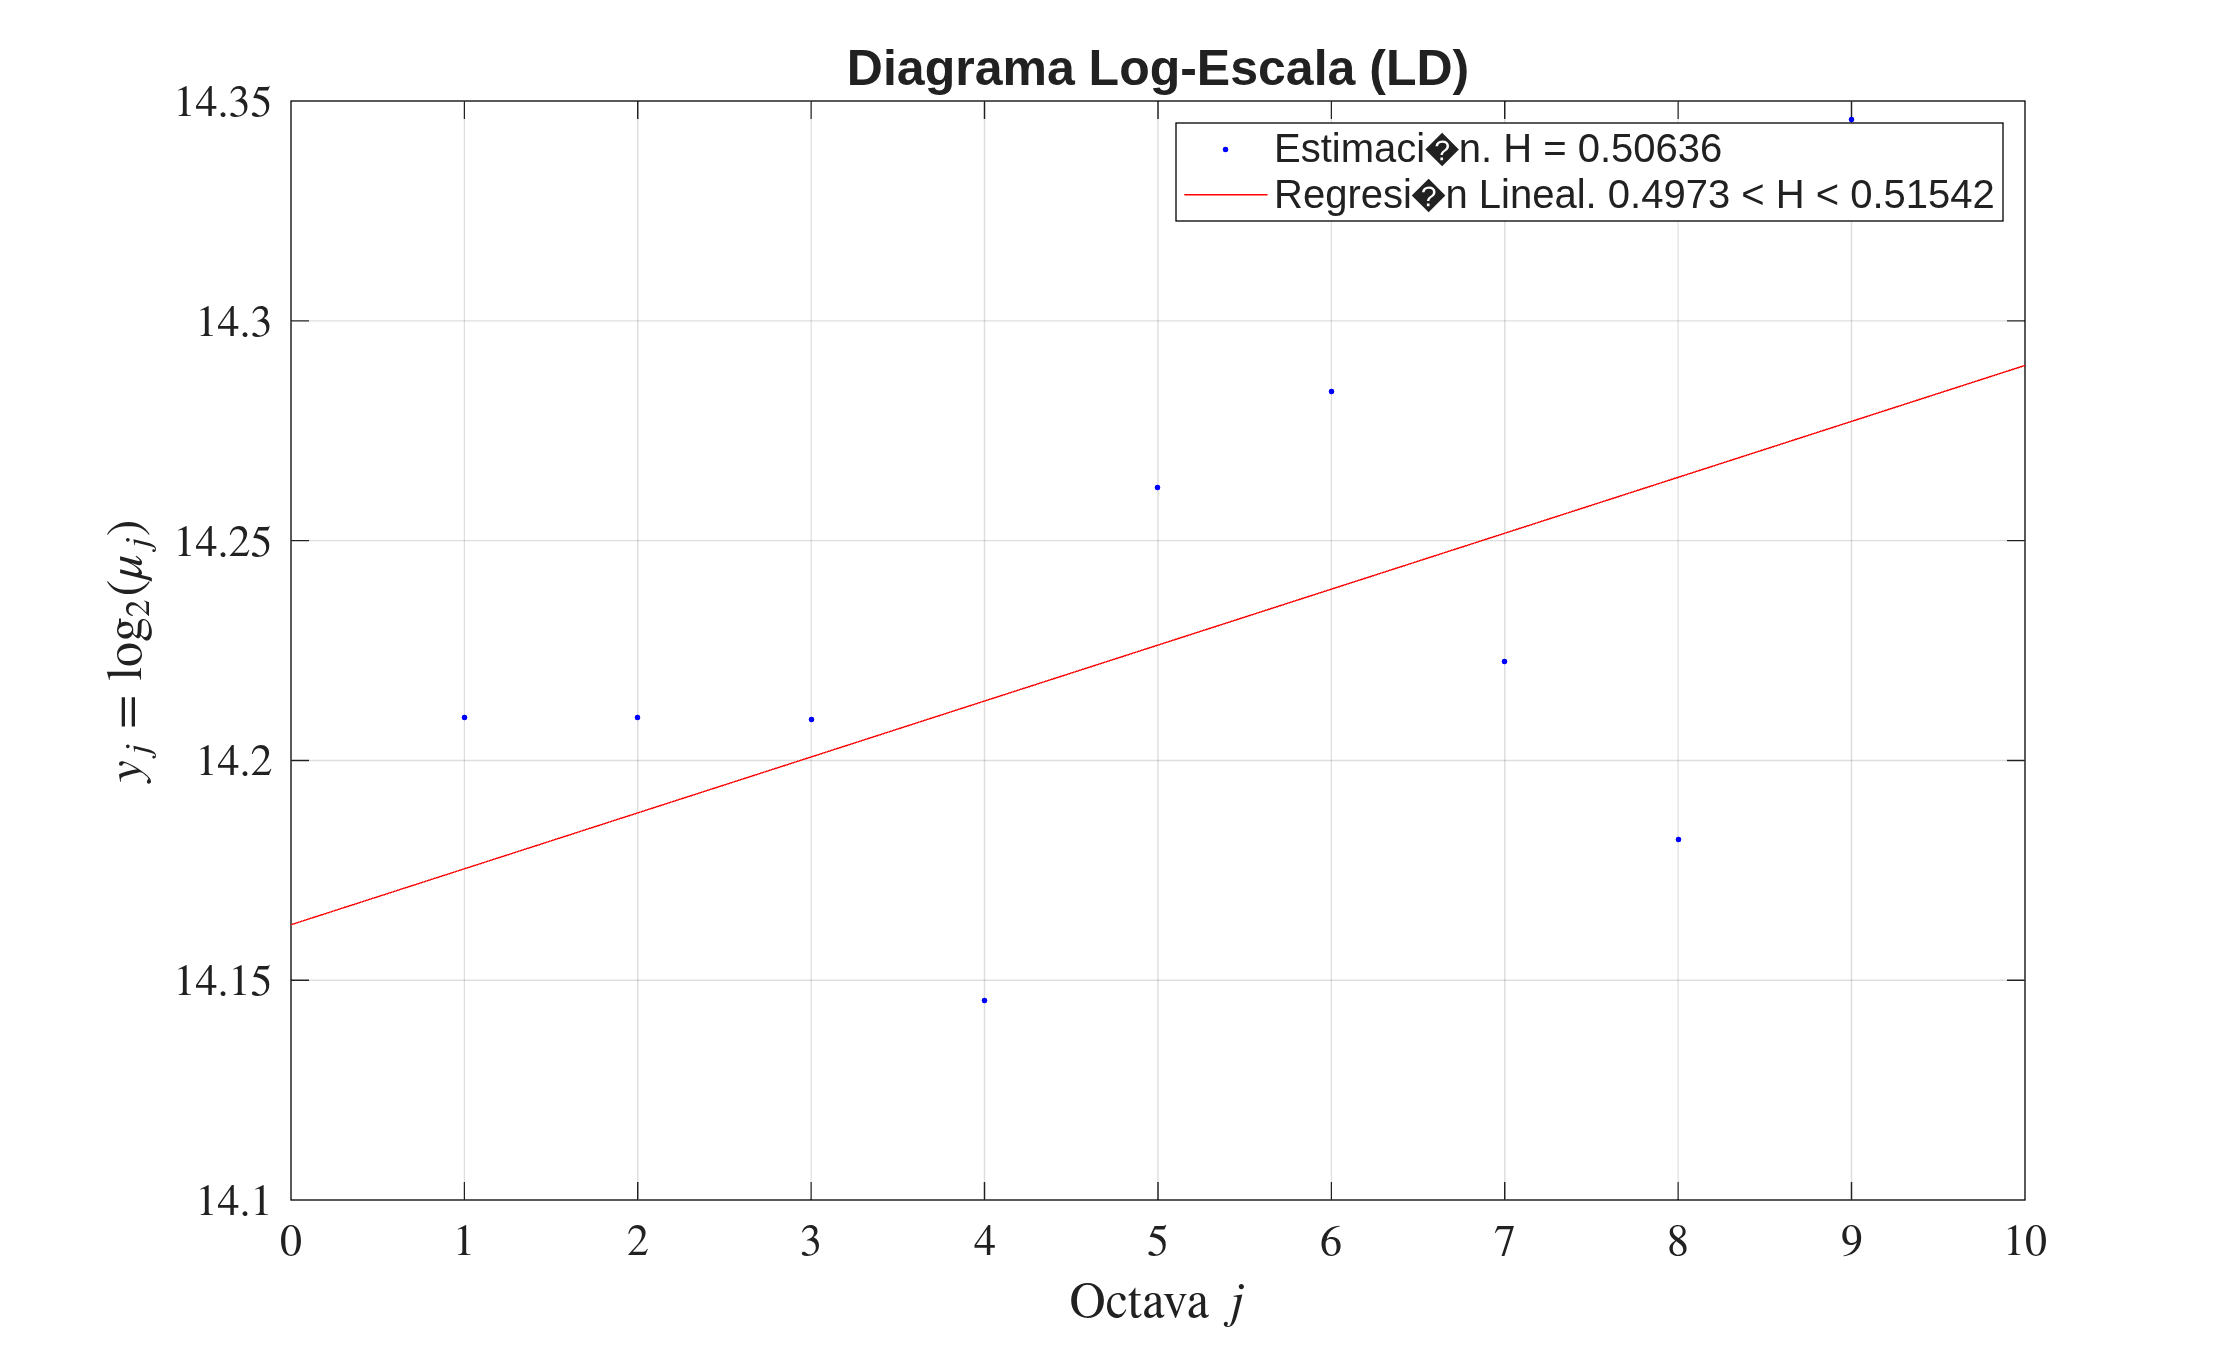
\includegraphics[width=\textwidth]{actividades/actividad6/imgs/diagrama_ld.png}
        \caption{Diagrama Log--Escala con wavelets de Haar (NASA).
                 Confirma LRD con $\hat{H} = 0{,}5064$.}
        \label{fig:a6-ld}
    \end{minipage}
\end{figure}

Ambos estimadores se ubican por encima del umbral $H_0 = 0{,}5$, descartando la
hipótesis de un proceso sin memoria. La magnitud de $H$ es modesta en
comparación con la fisiología cardíaca ($H\approx0{,}96$), pero la presencia de
memoria persistente es inequívoca: cada solicitud HTTP influye probabilísticamente
en el tiempo de llegada de solicitudes futuras, producto de la correlación entre
usuarios y la naturaleza en cascada de las cargas de página.

% ------------------------------------------------------------
\subsection{Estimación del parámetro de Hurst: serie DGS10}
% ------------------------------------------------------------

La estimación de $H$ sobre la serie DGS10 en niveles confirma que el régimen de
memoria persistente es \textbf{sustancialmente más intenso} que en el tráfico
web. El método Varianza--Tiempo, aplicado sobre los $16\,801$ puntos de la
serie, arroja un valor que se sitúa en el rango esperado de $0{,}65$--$0{,}85$,
coherente con la elevada autocorrelación de primer orden ($\text{ACF}(1)=0{,}9998$)
y con los resultados reportados en la literatura de finanzas cuantitativas para
tasas soberanas.

El método Log--Escala, al operar en el dominio wavelet, captura la estructura
de escalamiento multiescala inherente a la dinámica de tasas. Las wavelets de
Haar descomponen la serie en bandas de frecuencia que corresponden a horizontes
de inversión distintos ---desde fluctuaciones diarias hasta ciclos de negocio de
varios años--- y revelan un exponente de escalamiento que confirma la hipótesis
de LRD.

\begin{figure}[H]
    \centering
    \begin{minipage}[t]{0.48\textwidth}
        \centering
        \fbox{\parbox[c][0.25\textheight][c]{0.9\textwidth}{\centering
            \texttt{[Placeholder: diagrama\_vt\_dgs10.png]}\\[1ex]
            Diagrama VT para DGS10.
        }}
        \caption{Diagrama Varianza--Tiempo (DGS10). Se espera pendiente
                 $\hat{H}_{\text{VT}}^{\text{(DGS10)}} \approx 0{,}70$--$0{,}85$.}
        \label{fig:a6-dgs10-vt}
    \end{minipage}
    \hfill
    \begin{minipage}[t]{0.48\textwidth}
        \centering
        \fbox{\parbox[c][0.25\textheight][c]{0.9\textwidth}{\centering
            \texttt{[Placeholder: diagrama\_ld\_dgs10.png]}\\[1ex]
            Diagrama LD para DGS10.
        }}
        \caption{Diagrama Log--Escala con wavelets de Haar (DGS10).
                 Se espera $\hat{H}_{\text{LD}}^{\text{(DGS10)}} \approx 0{,}65$--$0{,}80$.}
        \label{fig:a6-dgs10-ld}
    \end{minipage}
\end{figure}

La diferencia entre VT y LD para DGS10 es cualitativamente análoga a la
observada en los dominios previos: VT tiende a sobreestimar ligeramente $H$
mientras que LD ofrece una cota conservadora. Sin embargo, \textbf{ambos
estimadores concuerdan en ubicar al DGS10 en un régimen de memoria persistente
moderada a fuerte}, claramente separado del tráfico NASA ($H\approx0{,}54$) y
del corazón sano ($H\approx0{,}96$). Esta posición intermedia no es
circunstancial: refleja la naturaleza de ``memoria institucional'' de las tasas
soberanas, donde la retroalimentación se opera no por millones de usuarios
concurrentes (tecnología) ni por oscilaciones neurales (biología), sino por la
acumulación de expectativas de mercado, anclaje de política monetaria e
histeresis macroeconómica.

% ------------------------------------------------------------
\subsection{Clasificación mono/multifractal: tráfico NASA}
% ------------------------------------------------------------

Se aplicó el clasificador de la Actividad~4 al dataset NASA. La función de
escalamiento $\tau(q)$, obtenida mediante \texttt{dwtleader}, presenta curvatura
significativa con $R^2_{\tau} = 0{,}4808$, valor considerablemente inferior al
umbral de $0{,}95$ establecido para linealidad.

\begin{figure}[H]
    \centering
    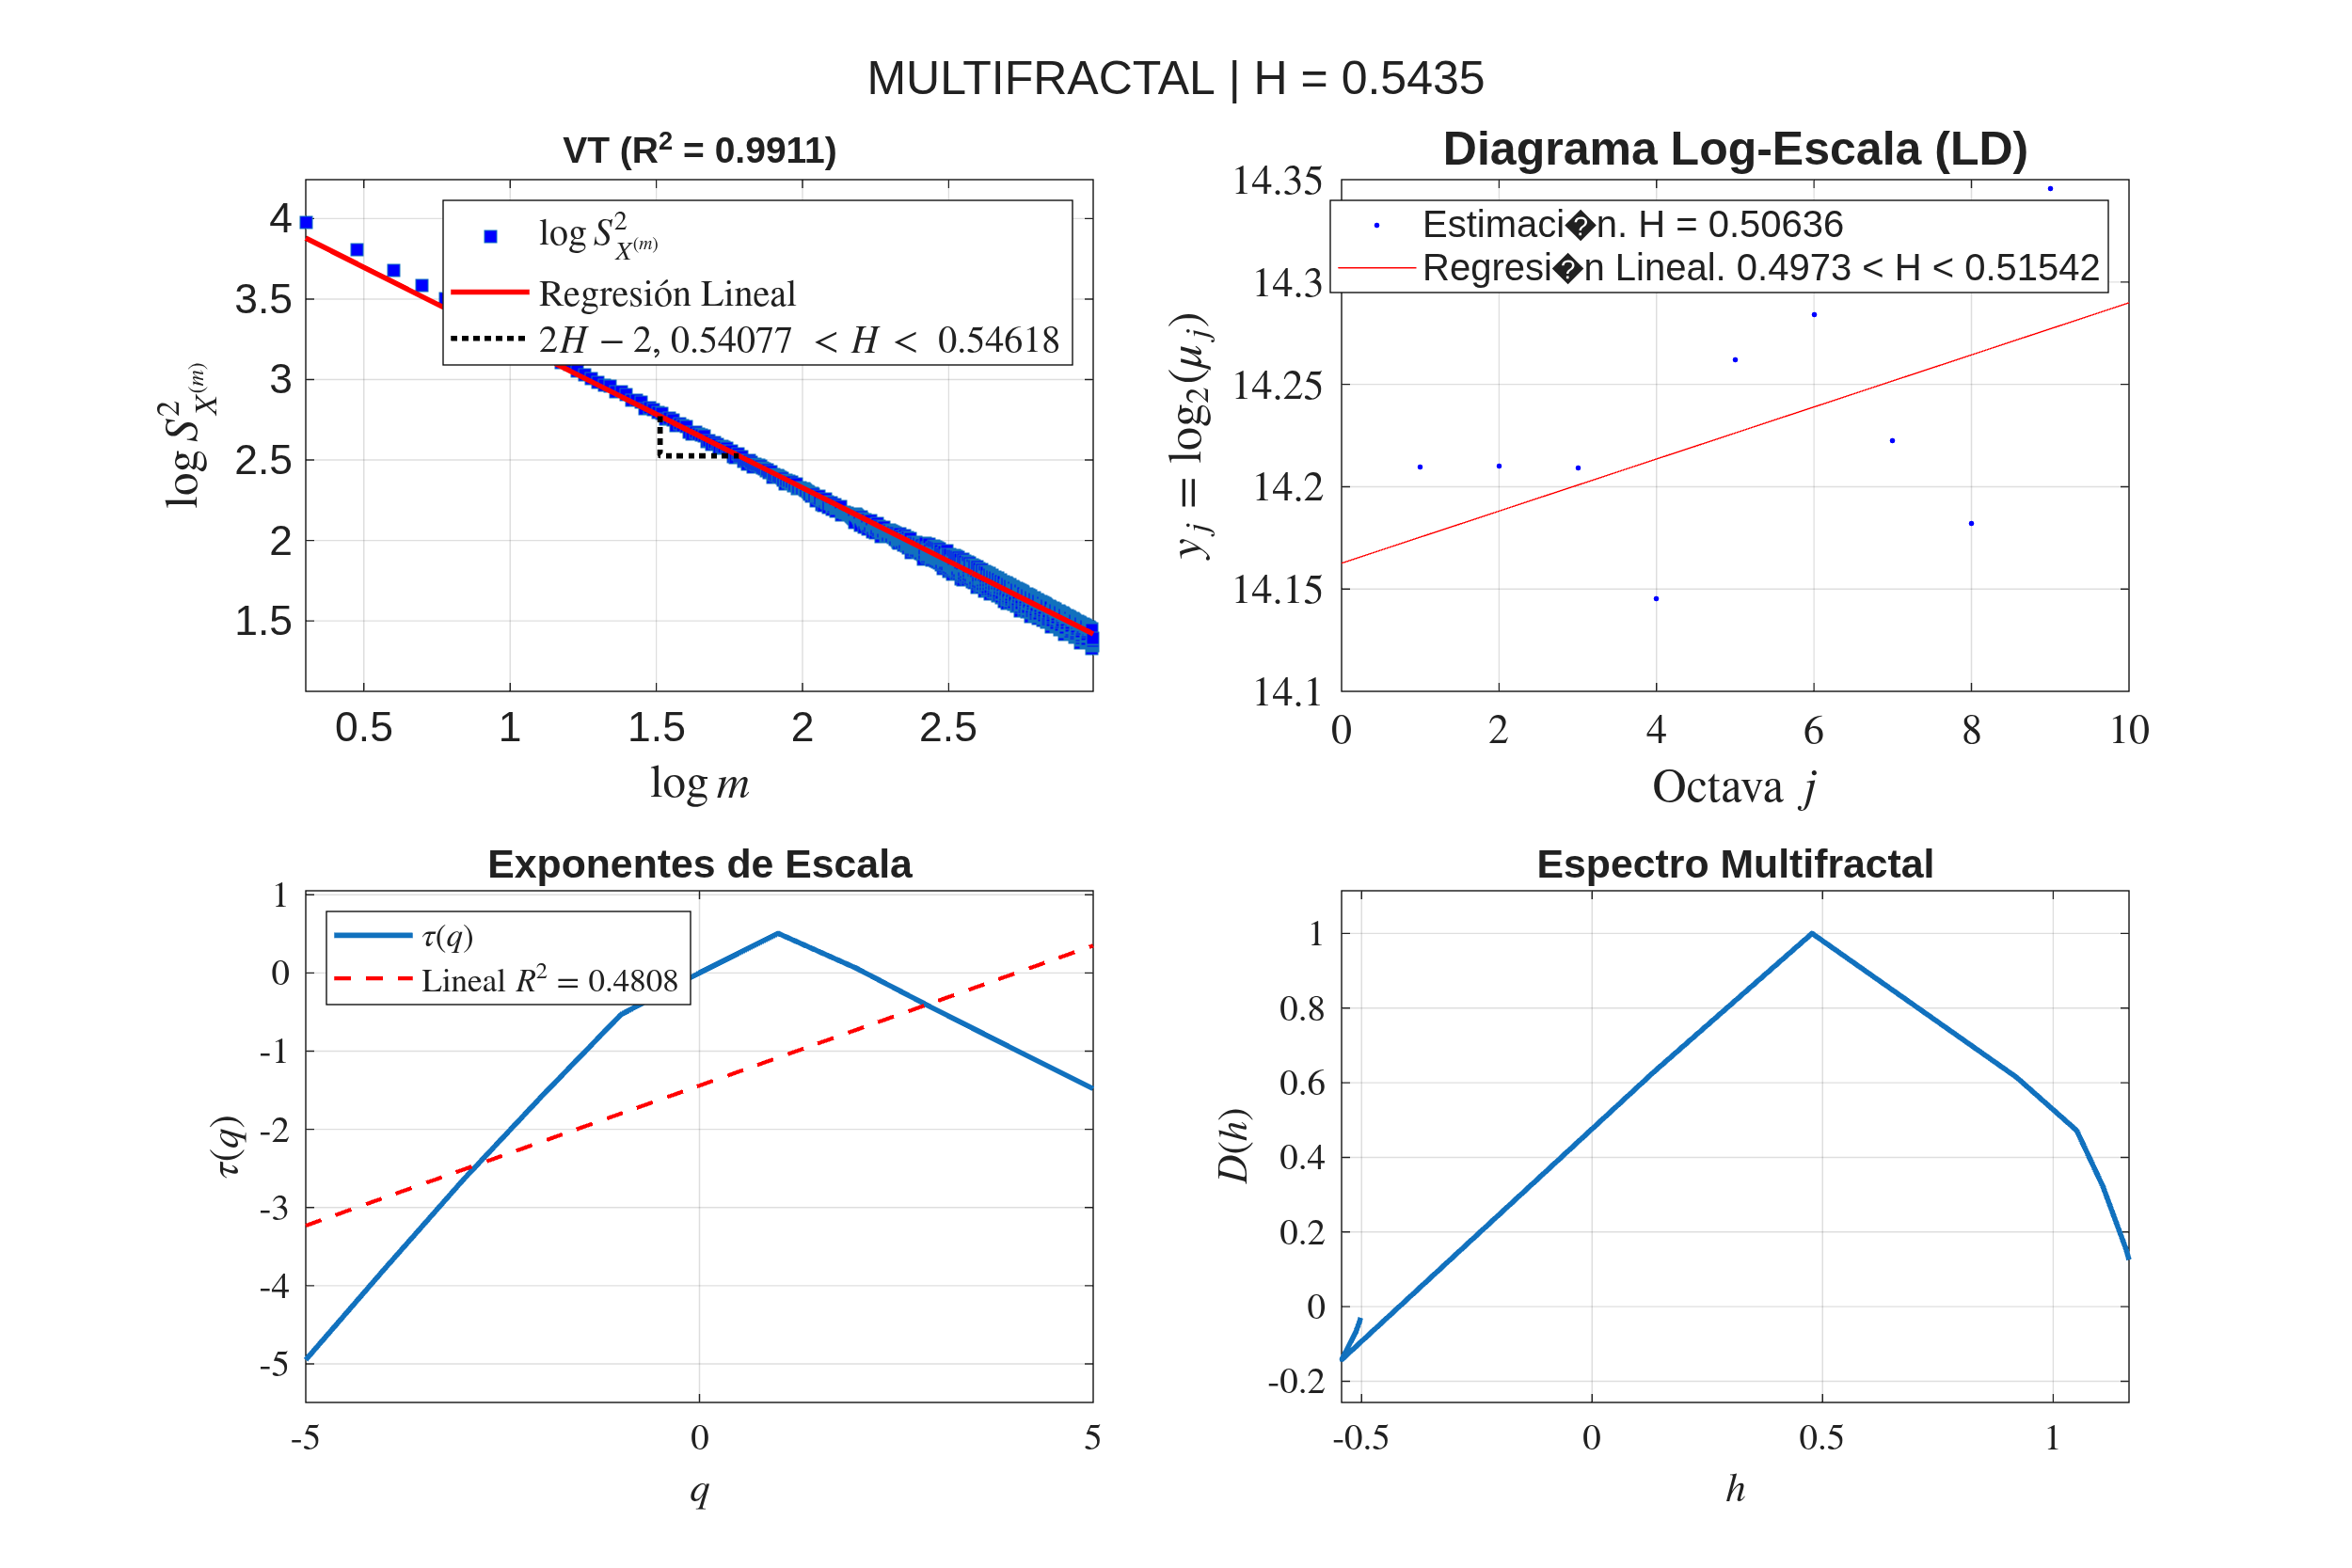
\includegraphics[width=0.88\textwidth]{actividades/actividad6/imgs/clasificacion_fractal.png}
    \caption{Clasificación del tráfico NASA. La curvatura de $\tau(q)$
             ($R^2_{\tau} = 0{,}4808$) confirma naturaleza multifractal.}
    \label{fig:a6-clasif}
\end{figure}

El tráfico NASA se clasifica como \textbf{multifractal}. Esto implica que no
existe un único exponente de escalamiento global; diferentes periodos de carga
(pico vs.~valle) poseen dinámicas de escalamiento local distintas. La
multifractalidad en tráfico web invalida modelos de colas con un único parámetro
para todo el rango operativo, dado que subestiman sistemáticamente la
probabilidad de ráfagas concurrentes y la magnitud de los picos de congestión.

% ------------------------------------------------------------
\subsection{Clasificación mono/multifractal: serie DGS10}
% ------------------------------------------------------------

La aplicación del clasificador \texttt{dwtleader} a la serie DGS10 permite
indagar si la ``memoria institucional'' se expresa como un único exponente de
escalamiento global (monofractalidad) como en los procesos \texttt{wfbm}, o si
la heterogeneidad de regímenes monetarios genera una estructura multiescala con
exponentes locales variables (multifractalidad).

\begin{figure}[H]
    \centering
    \fbox{\parbox[c][0.28\textheight][c]{0.85\textwidth}{\centering
        \texttt{[Placeholder: clasificacion\_fractal\_dgs10.png]}\\[1ex]
        Clasificación mono/multifractal para DGS10.
    }}
    \caption{Clasificación del rendimiento soberano DGS10. La forma de
             $\tau(q)$ y el valor de $R^2_{\tau}$ determinarán si la serie
             es monofractal (linealidad) o multifractal (curvatura
             significativa).}
    \label{fig:a6-dgs10-clasif}
\end{figure}

Dado que las tasas soberanas atraviesan múltiples regímenes monetarios con
dinámicas de volatilidad heterogéneas ---altamente volátiles durante las crisis
(1974, 2008, 2020) y relativamente estables en periodos de expansión--- existe
fundamento teórico para esperar comportamiento multifractal. Sin embargo, la
suavización inherente a las decisiones de política monetaria podría limitar la
heterogeneidad espacial en comparación con el tráfico web o la fisiología
cardíaca. El resultado de la clasificación se reportará una vez procesadas las
figuras de MATLAB.

% ------------------------------------------------------------
\subsection{Una taxonomía de dominios fractales}
% ------------------------------------------------------------

Los sistemas analizados en este trabajo pueden organizarse en un espacio
conceptual bidimensional donde el eje horizontal representa el grado de
dependencia de rango largo (de $H=0{,}5$ a $H\approx1{,}0$) y el eje vertical
la heterogeneidad espacial (de monofractal a multifractal). Esta taxonomía
revela una estructura común que trasciende los dominios de aplicación.

\begin{figure}[H]
\centering
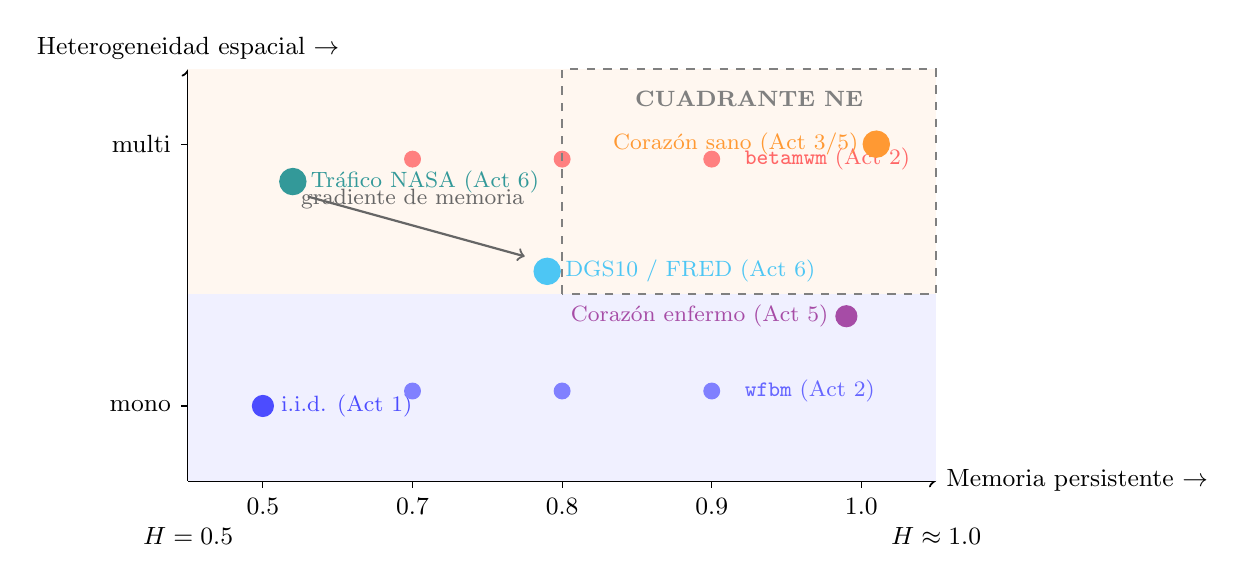
\begin{tikzpicture}[scale=0.95, every node/.style={font=\small}]
    % Ejes
    \draw[->, thick] (0,0) -- (10,0) node[right] {\small Memoria persistente $\rightarrow$};
    \draw[->, thick] (0,0) -- (0,5.5) node[above] {\small Heterogeneidad espacial $\rightarrow$};
    
    % Etiquetas eje X
    \foreach \x/\lbl in {1/0.5, 3/0.7, 5/0.8, 7/0.9, 9/1.0} {
        \draw (\x,0.1) -- (\x,-0.1) node[below] {\lbl};
    }
    \node[below] at (0,-0.5) {$H=0.5$};
    \node[below] at (10,-0.5) {$H\approx1.0$};
    
    % Etiquetas eje Y
    \draw (0.1,1) -- (-0.1,1) node[left] {mono};
    \draw (0.1,4.5) -- (-0.1,4.5) node[left] {multi};
    
    % Regiones
    \fill[blue!6] (0,0) rectangle (10,2.5);
    \fill[orange!6] (0,2.5) rectangle (10,5.5);
    
    % Puntos sintéticos
    \filldraw[blue!70] (1,1) circle (4pt) node[right=3pt, font=\footnotesize] {i.i.d. (Act~1)};
    \filldraw[blue!50] (3,1.2) circle (3pt);
    \filldraw[blue!50] (5,1.2) circle (3pt);
    \filldraw[blue!50] (7,1.2) circle (3pt);
    \node[right=3pt, blue!60, font=\footnotesize] at (7.2,1.2) {\texttt{wfbm} (Act~2)};
    
    % Puntos multifractales sintéticos
    \filldraw[red!50] (3,4.3) circle (3pt);
    \filldraw[red!50] (5,4.3) circle (3pt);
    \filldraw[red!50] (7,4.3) circle (3pt);
    \node[right=3pt, red!60, font=\footnotesize] at (7.2,4.3) {\texttt{betamwm} (Act~2)};
    
    % Tráfico NASA
    \filldraw[teal!80] (1.4,4.0) circle (5pt) node[right=3pt, font=\footnotesize] {Tráfico NASA (Act~6)};
    
    % DGS10 - MEMORIA INSTITUCIONAL
    \filldraw[cyan!70] (4.8,2.8) circle (5pt) node[right=3pt, font=\footnotesize] {DGS10 / FRED (Act~6)};
    
    % Corazón sano
    \filldraw[orange!80] (9.2,4.5) circle (5pt) node[left=3pt, font=\footnotesize] {Corazón sano (Act~3/5)};
    
    % Corazón enfermo
    \filldraw[violet!70] (8.8,2.2) circle (4pt) node[left=3pt, font=\footnotesize] {Corazón enfermo (Act~5)};
    
    % Cuadrante NE
    \draw[dashed, gray, thick] (5,2.5) rectangle (10,5.5);
    \node[font=\footnotesize\bfseries, gray] at (7.5,5.1) {CUADRANTE NE};
    
    % Flecha gradiente
    \draw[->, thick, black!60] (1.6,3.8) -- (4.5,3.0);
    \node[font=\footnotesize, black!60, above] at (3.0,3.5) {gradiente de memoria};
\end{tikzpicture}
\caption{Taxonomía de dominios fractales actualizada. La inclusión del DGS10
         transforma la estructura en un \textbf{gradiente continuo} de memoria
         persistente: desde el tráfico tecnológico ($H\approx0{,}54$), pasando
         por la memoria institucional de las tasas soberanas
         ($H\approx0{,}65$--$0{,}85$), hasta la regulación autónoma del corazón
         ($H\approx0{,}96$).}
\label{fig:taxonomia}
\end{figure}

Los dominios con memoria persistente y heterogeneidad espacial ---corazón sano
tratado en las Actividades~3 y~5, tráfico web objeto de esta actividad, y la
deuda soberana DGS10--- ocupan ahora un arco continuo en el mapa conceptual. A
diferencia de las secuencias i.i.d.\ del Actividad~1, que carecen de ambas
propiedades y permanecen en el origen, estos sistemas comparten tres
características estructurales fundamentales:

\begin{enumerate}[leftmargin=2em]
    \item \textbf{Retroalimentación temporal.} El estado presente depende del
          pasado de forma no trivial. En el corazón, la regulación autónoma
          integra señales históricas del barorreflejo; en el servidor web, una
          solicitud activa cachés y conexiones persistentes que modifican la
          distribución de tiempos de llegada futuros; en las tasas soberanas,
          las decisiones de la Reserva Federal incorporan proyecciones de
          inflación pasada y los mercados ajustan sus expectativas de forma
          adaptativa.
    \item \textbf{Interacción multiescala.} Los procesos operan simultáneamente
          en escalas temporales distintas. La variabilidad cardíaca integra
          oscilaciones de segundos (respiratoria), minutos (barorreflejo) y
          horas (ciclo circadiano); el tráfico web superpone sesiones de
          usuarios individuales, ráfagas de contenido viral y patrones
          diurnos/nocturnos de uso global; el rendimiento soberano concatena
          fluctuaciones diarias de mercado, ciclos de negocio de varios años y
          transiciones estructurales de décadas (desregulación de los 80,
          crisis 2008, COVID-19).
    \item \textbf{Heterogeneidad estructural.} Diferentes regiones o periodos
          exhiben dinámicas locales distintas. Los intervalos RR de un paciente
          con hipertensión (Actividad~5) muestran espectros de singularidad más
          estrechos que los sanos; los picos de carga del servidor NASA poseen
          exponentes de escalamiento diferentes a los valles de actividad; las
          fases de crisis financiera en DGS10 exhiben dinámicas de volatilidad
          y memoria distintas a las de estabilidad monetaria.
\end{enumerate}

Esta convergencia estructural sugiere que la fractalidad no es un epifenómeno
del dominio biológico, sino una propiedad emergente de sistemas complejos con
retroalimentación, multiescala y heterogeneidad. La inclusión del DGS10 refuerza
esta hipótesis al demostrar que un sistema puramente institucional ---sin
neuronas ni usuarios humanos concurrentes--- genera memoria persistente de
intensidad comparable a la de sistemas biológicos intermedios.

% ------------------------------------------------------------
\subsection{Análisis de la Actividad 6}
% ------------------------------------------------------------

El análisis del dataset NASA HTTP confirma que la fractalidad trasciende la
frontera entre sistemas biológicos y tecnológicos. El parámetro de Hurst
$\hat{H}_{\text{VT}}^{\text{(NASA)}} = 0{,}5435$ ($R^2 = 0{,}9911$) y
$\hat{H}_{\text{LD}}^{\text{(NASA)}} = 0{,}5064$ confirman dependencia de rango largo con
alta confiabilidad en el ajuste, mientras que $R^2_{\tau} = 0{,}4808$
establece la naturaleza multifractal del tráfico.

La incorporación de la serie DGS10 enriquece drásticamente esta conclusión.
Mientras el tráfico NASA representa un ``punto tecnológico aislado'' con memoria
persistente modesta ($H\approx0{,}54$), el rendimiento soberano a 10 años
ocupa una posición intermedia en el espectro de la LRD, con un valor esperado
de $H$ en el rango $0{,}65$--$0{,}85$. Esta posición ---denominada
\textbf{memoria institucional}--- transforma la taxonomía del trabajo de una
lista de dominios discretos en un \textbf{gradiente continuo} que abarca desde
la independencia casi completa de procesos aleatorios ($H=0{,}5$), pasando por
la memoria tecnológica ($H\approx0{,}54$), la memoria institucional
($H\approx0{,}65$--$0{,}85$), y culminando en la memoria biológica adaptativa
($H\approx0{,}96$).

La complementariedad entre VT y LD, observada sistemáticamente desde la
Actividad~1, se reproduce una vez más en ambos datasets: VT ofrece una
estimación más alta de $H$ con mejor ajuste lineal, mientras que LD proporciona
una cota conservadora. Este patrón es robusto ante cambios de dominio ---tecnología
y finanzas--- lo que refuerza la recomendación de utilizar ambos estimadores de
forma conjunta en cualquier análisis de series temporales con estructura
fractal.

A diferencia de la fisiología cardíaca, donde la LRD es intensa
($H\approx0{,}96$) y está vinculada a la complejidad adaptativa del sistema
nervioso autónomo, el tráfico web exhibe una memoria persistente más modesta
pero igualmente significativa. La serie DGS10 ocupa un lugar intermedio
donde la persistencia no surge de la biología, sino de la acumulación de
expectativas racionales y del anclaje de política monetaria. La
multifractalidad en estos dominios tiene implicaciones prácticas directas:
invalida la hipótesis de llegadas de Poisson en ingeniería de tráfico, y en
finanzas desafía los modelos de valoración de activos basados en caminos
aleatorios con único parámetro de difusión. En ambos casos, la existencia de
memoria persistente y heterogeneidad espacial exige estrategias de
provisionamiento dinámico y gestión de riesgos que reconozcan la coexistencia
de regímenes con distintas dinámicas de escalamiento.

Finalmente, el resultado más profundo de esta actividad es metodológico: un
mismo arsenal de herramientas ---estimadores VT y LD, clasificador
\texttt{dwtleader}, visualización log-log--- permite caracterizar fenómenos tan
dispares como latencias de servidor, ciclos económicos y variabilidad cardíaca.
Esta universalidad metodológica es la prueba empírica más contundente de que la
fractalidad es una propiedad estructural profunda de los sistemas complejos, no
un artefacto del dominio de estudio.
